\FloatBarrier
\section{یادگیری عمیق}\label{ch:literature-review|sec:deep-learning}


با توسعه‌ی الگوریتم های یادگیری ماشین و یادگیری عمیق در حوزه های مختلف فناوری و مهندسی، بازسازی تصاویر \mri نیز از این مقوله مستثنا نبوده است. اخیرا مقالات زیادی در این زمینه با استفاده از یادگیری عمیق انجام شده است. 

\begin{figure}[t!]
	\centering
	\begin{copyrightBox}{\linewidth}{\Doi{10.1109/tmi.2019.2927101}}
	\subfigure[]{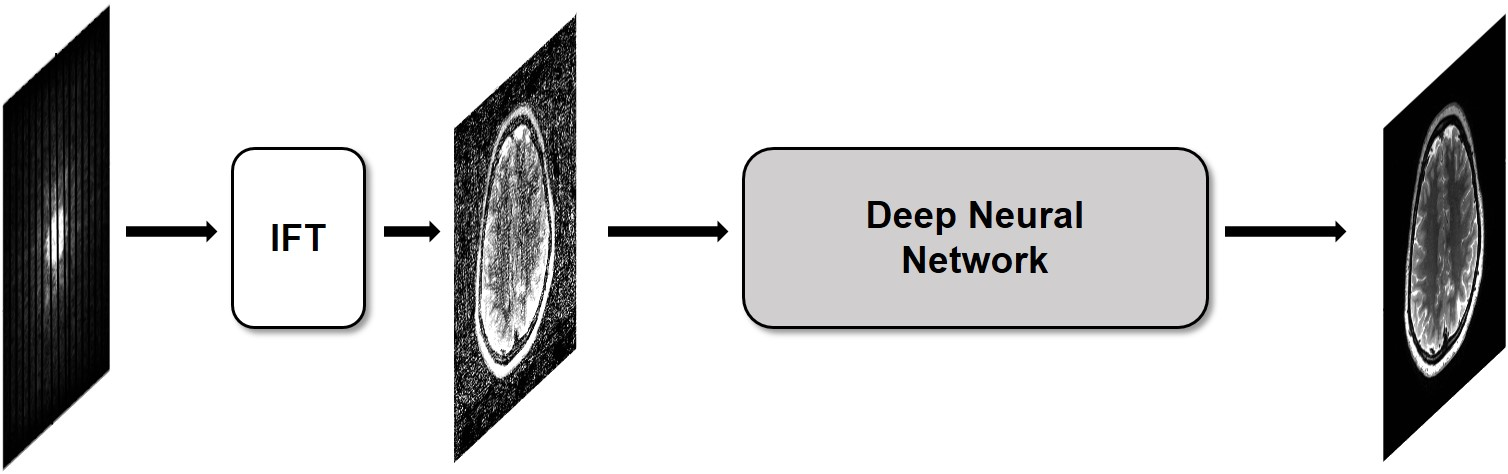
\includegraphics[width=0.4\linewidth]{chapters/chapter-3/figs/deep-learning_a}}
	\hspace{0.1\linewidth}
	\subfigure[]{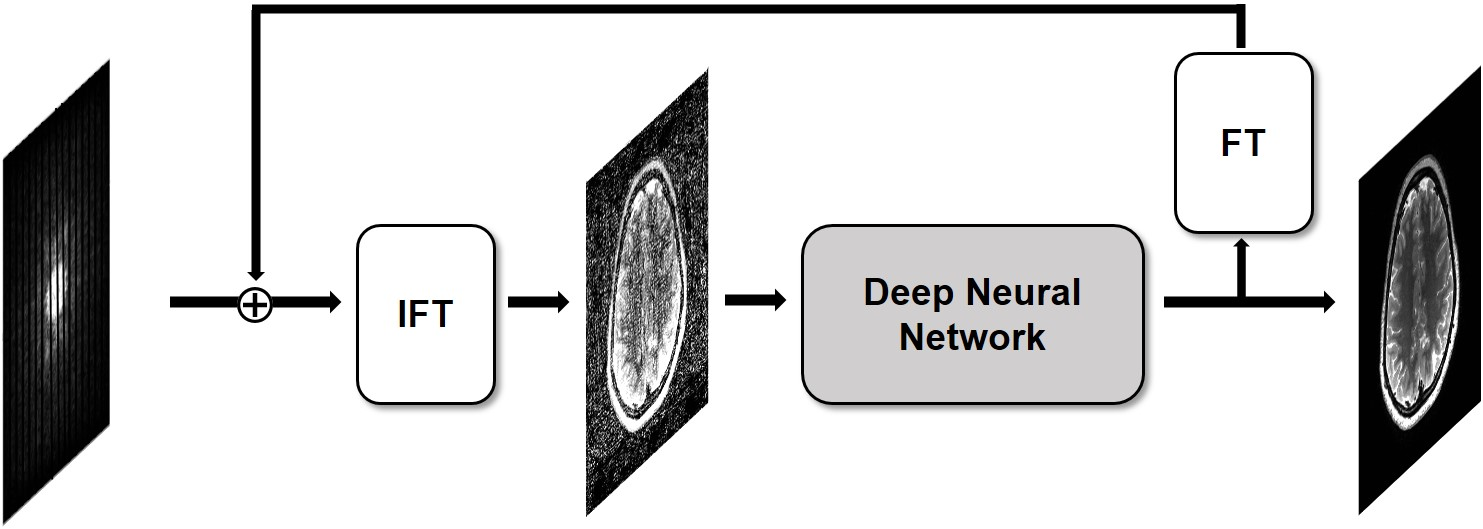
\includegraphics[width=0.4\linewidth]{chapters/chapter-3/figs/deep-learning_b}}
	
	\subfigure[]{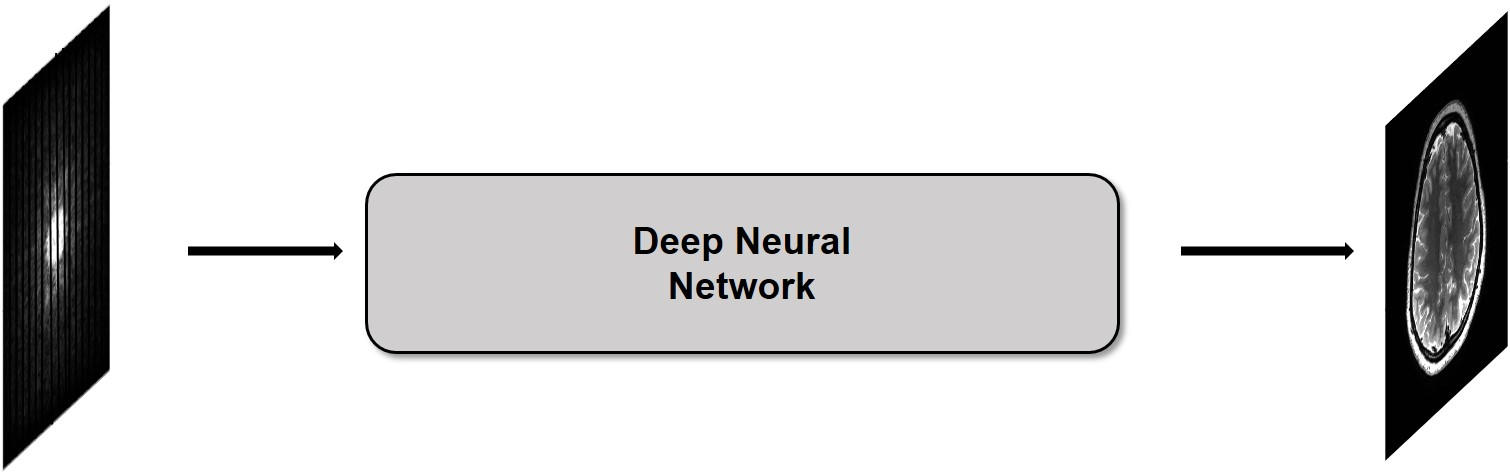
\includegraphics[width=0.4\linewidth]{chapters/chapter-3/figs/deep-learning_c}\label{subfig:deep-learning-c}}
	\hspace{0.1\linewidth}
	\subfigure[]{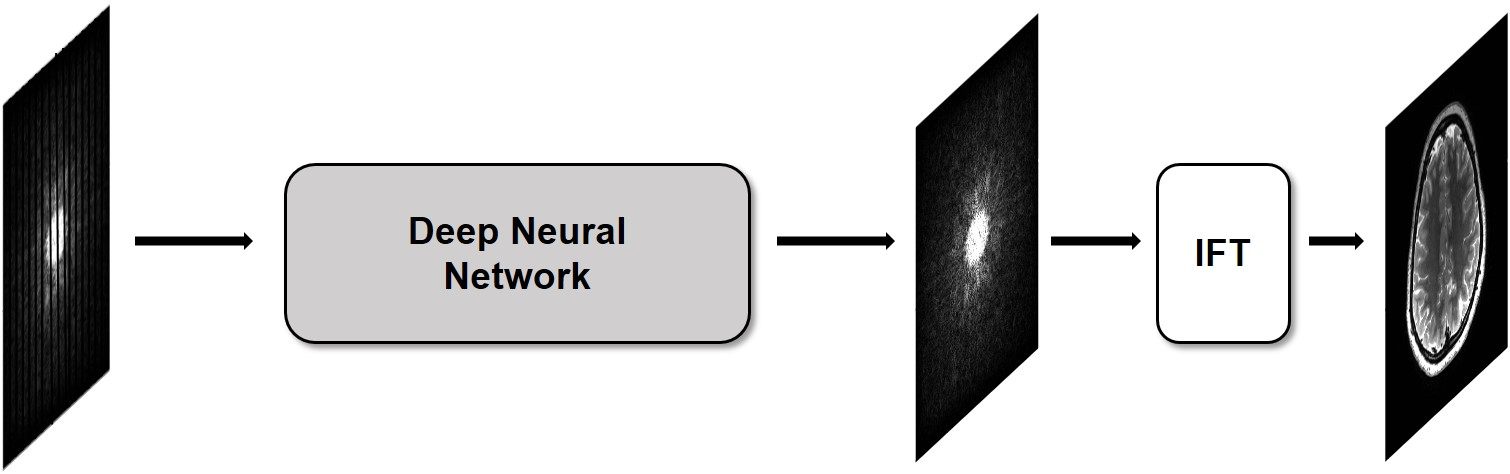
\includegraphics[width=0.4\linewidth]{chapters/chapter-3/figs/deep-learning_d}}
	\end{copyrightBox}
	\removevspace
	\caption{}
	\label{fig:deep-learning-model}
\end{figure}


روش کلی در تمامی این مقالات این است که با داشتن داده های کامل نمونه برداری شده
\LTRfootnote{fully-sampled data}
و \kspace متناظر‌ آن، ابتدا داده هایی با نرخ کمتر تولید می‌کنند و سپس این جفت دادگان را به یک شبکه یاد‌گیری ماشین می‌دهند به گونه ای که سیستم طراحی شده در ورودی خود دادگان \kspace نمونه برداری شده با نرخ کمتر و در خروجی خود تصویر \mri با نرخ نمونه برداری کامل را ببیند و سیستم طراحی شده سعی کند که رابطه بین ورودی و خروجی را کشف کند.
شکل \ref{fig:deep-learning-model}
به نقل از \cite{kSpace-deeplearning2020}
حالت های ممکن مورد بررسی در این روش‌ها را بیان ‌می‌کند.










\subsection{استفاده از اتوانکدور در حوزه‌ی \kspace}
تبدیل فوریه مکانی
\LTRfootnote{Spatial Fourier Transform}
یک سیگنال دلخواه
$x \colon \mathbb{R}^2 \rightarrow \mathbb{R} $




\removevspace
\begin{equation}
	\hat{x}(\mathbf{k})=\mathcal{F}[x](\mathbf{k}):=\int_{\mathbb{R}^{d}} e^{-\iota \mathbf{k} \cdot \mathbf{r}} x(\mathbf{r}) d \mathbf{r}
\end{equation}

\removevspace
\begin{equation}
	\mathbf{y} = \mathcal{P}_{\Lambda}[\hat{\mathbf{x}}]
\end{equation}

\removevspace
\begin{equation}
	\left[\mathcal{P}_{\Lambda}[\hat{\mathbf{x}}]\right]_{i}= 
	\begin{cases}
		\hat{x}[i], & i \in \Lambda \\ 
		0, & \rltext {سایر موارد}
	\end{cases}
\end{equation}

\removevspace
\begin{equation}
	\widehat{\mathbf{x}}=[\hat{x}[0] \quad \cdots \quad \hat{x}[N-1]], \qquad \text { where } \quad \hat{x}[i]=\widehat{x}\left(\mathbf{k}_{i}\right)
\end{equation}




در ساختار \lr{CS-MRI} تلاش می‌شود که مسئله‌ی بهینه سازی زیر حل شود تا از اسپارسیتی در یک حوزه تبدیل بتوان به منظور بازسازی تصویر از روی نقاط باقیمانده کند. مشکل اصلی این کار که در مقاله \cite{Lustig_2007} راه حل حسگری فشرده آن مورد بررسی قرار گرفت، این است که به بخاطر مفهوم مطلوب ناهمدوستی
\LTRfootnote{Incoherency}
مجبور به آپدیت کردن بین هردو حوزه‌ی تصویر و حوزه \kspace است.

\removevspace
\begin{subequations}
	\begin{align}
		\min_{\hat{z}\in\mathbb{C}^N} \ \ &\|\mathcal{T}z\|_1 \\
		\lrtext{s.t.} \ \ & \Rho_\Lambda([\hat{x}]) = \Rho_\Lambda([\hat{z}])
	\end{align}
\end{subequations}

همان‌گونه که در بخش \ref{ch:literature-review|sec:compressed-sensing|subsec:aloha} نیز توضیح داده شد،
مقاله \cite{Jin_2016}
توانست نشان دهد که بین اسپارسیتی در یک حوزه تبدیل از تصویر (یا
\lr{FRI}\LTRfootnote{Finite Rate Inovation})
و حوزه \kspace ارتباطی وجود دارد و این ارتباط به رنک پایین بودن
\LTRfootnote{Low-Rankness}
ماتریس ساختاریافته هنکل
\LTRfootnote{Structured Hankel Matrix}
در حوزه \kspace بر میگردد. به عبارت دیگر اگر سیگنال ورودی یک سیگنال \lr{FRI} باشد، ماتریس ساختار یافته هنکل آن در حوزه فوریه، رنک پایین خواهد بود.

بنابراین مسیله‌ی \lr{CS-MRI}
را می‌توان به شکل زیر در آورد که در \cite{Jin_2016} از آن به نام \lr{ALOHA} یاد برده است.



\removevspace
\begin{subequations}
	\begin{align}
		\min_{\hat{z}\in\mathbb{C}^N} \ &\mathrm{Rank}(\mathcal{H}_d(\hat{z})) \\
		\lrtext{s.t.} \ & \Rho_\Lambda([\hat{x}]) = \Rho_\Lambda([\hat{z}])
	\end{align}
\end{subequations}


حال میخواهیم این مسيله را به یک مسیله یادگیری عمیق 
\LTRfootnote{Deep-Learning}
تبدیل کنیم. از آنجایی که ما از ساختار شکل \ref{subfig:deep-learning-c}
استفاده می‌کنیم، مساعد است که یک تابع هزینه را روی حوزه تصویر تشکیل دهیم از این رو الگوریتم \lr{ALOHA} را به شکل زیر ویرایش می‌کنیم.


\removevspace
\begin{subequations}\label{eq:aloha-modify1}
	\begin{align}
		\min_{\hat{z}\in\mathbb{C}^N} \ \  & \| x - \F^{-1}{\hat{z}}\| \\
		\lrtext{s.t.} \ \  & \mathrm{Rank}(\mathcal{H}_d(\hat{z})) = s, \\
		& \Rho_\Lambda([\hat{x}]) = \Rho_\Lambda([\hat{z}])
	\end{align}
\end{subequations}

که در آن $s$ یک تخمینی از رنک ماتریس ساختار یافته هنکل است. توجه داریم که تابع
$\mathrm{Rank}(.)$
یک قید غیر کانوکس 
\LTRfootnote{non-convex}
است. در مقاله \cite{Jin_2016}
به پیشنهاد از روش تکمیل ماتریس 
\cite{Cand_s_2009}
استفاده از رنک هسته‌ای
\LTRfootnote{nuclear norm}
را برای حل این مشکل توصیه کرده است اما این مقاله روش دیگری را برای غلبه بر این مشکل را اتخاذ کرده است. 

در ابتدا از اعداد مختلط خود را خلاص می‌کنیم. این کار به سادگی با تعریف اپراتور $\Re(z): \mathbb{C}\rightarrow\mathbb{R}^2$
روبرو امکان پذیر است:
$\Re(z) = [\mathcal{Re}(z) \mathcal{Im}(z)]$

در این صورت می‌توان معادله \ref{eq:aloha-modify1}
را به صورت زیر با نویسی نمود.

\removevspace
\begin{subequations}
	\begin{align}
		\min_{\hat{z}\in\mathbb{C}^N} \ \  & \| x - \F^{-1}{\hat{z}}\| \\
		\lrtext{s.t.} \ \  & \mathrm{Rank}(\mathcal{H}_{d|2}(\Re(\hat{z}))) = Q \le 2s, \\ 
		& \Rho_\Lambda([\hat{x}]) = \Rho_\Lambda([\hat{z}])
	\end{align}
\end{subequations}

حال می خواهیم آن را به فرم یادگیری عمیق در بیاوریم. برای این کار چون از ساختار   \ref{subfig:deep-learning-c} استفاده کردیم و در این ساختار ورودی و خروجی، حوزه ای یکسان دارند،  پس می‌توان از یک ساختار متقارن اتوانکودر
\LTRfootnote{Auto-encoder}
استفاده کرد.
که دارای المان های پولینگ
\LTRfootnote{Pooling}
و آنپولینگ
\LTRfootnote{Unpooling}
است. این مقاله سعی میکند که آن قید رنک را در درون ساختار شبکه تزریق کند تا همیشه برآورده شود.

تجزیه \lr{SVD} ماتریس 
$\mathcal{H}_d(\Re(\hat{z})) =  U \Sigma V^T$
را در نظر بگیرد. میتوان دو بردار 
$\Psi, \tilde{\Psi} \in \mathbb{R}^{2d\times Q}$
را به نحوی تعریف کرد که حاصل ضرب آن 
$\Psi\tilde{\Psi}^T = P_{\mathrm{Range}(V)}$
شود. در این رابطه $P_{\mathrm{Range}(V)}$ ماتریس پروجکشن روی برد ماتریس $V$ حاصل از تجزیه \lr{SVD}
مذکور خواهد بود. همچنین ماتریس های پولینک و آنپولینگ 
$\Phi, \tilde{\Phi} \in \mathbb{R}^{M\times N}$
را تعریف کرد. چون که شبکه متقارن است پس میتوان عملکرد این دو را معکوس هم به شکل 
$\Phi\tilde{\Phi}^T = I_{N}$
دانست. از این رو روابط زیر را میتوان استخراج نمود.



\removevspace
\begin{equation}
	\mathcal{H}_{d|2}(\Re(\hat{z})) = \Phi\tilde{\Phi}^T \mathcal{H}_{d|2}(\Re(\hat{z})) \Psi\tilde{\Psi}^T = \Phi \mathbf{C} \tilde{\Psi}^T \\
\end{equation}
که در آن
\removevspace
\begin{equation}
	\mathbf{C} \coloneqq \tilde{\Phi}^T \mathcal{H}_{d|2}(\Re(\hat{z})) \Psi
\end{equation}

حال می‌توان فضای برداری $\mathcal{H}$
را به صورت زیر تعریف کرد.

\removevspace
\begin{equation}
	\begin{aligned}
		\mathcal{H}(\boldsymbol{\Psi}, \tilde{\boldsymbol{\Psi}})=&\left\{\mathbf{z} \in \mathbb{C}^{N} \mid \Re[\mathbf{z}]=\boldsymbol{\Phi}^{\top}(\mathbf{C} \circledast g(\tilde{\boldsymbol{\Psi}}))\right.\\
		&\mathbf{C}=(\tilde{\boldsymbol{\Phi}} \Re[\mathbf{z}]) \circledast h(\boldsymbol{\Psi})\}
	\end{aligned}
\end{equation}

با این تعریف میخواهیم بهینه سازی را صرفا بر روی این فضا حل کنیم. بنابراین این مسیله به صورت زیر قابل بازنویسی است.

\removevspace
\begin{subequations}\label{eq:P'A}
	\begin{align}
		(P'_A) \quad
		\min_{\hat{z}\in\mathbb{\mathcal{H}(\psi, \tilde{\psi})}} \ \
		\min_{\Psi, \tilde{\Psi}} \ \  & \| x - \F^{-1}{\hat{z}}\| \\
		\lrtext{s.t.} \quad  & \Rho_\Lambda([\hat{x}]) = \Rho_\Lambda([\hat{z}])
	\end{align}
\end{subequations}


حال با این تعریف میتوان شبکه کانوولوشنالی های در یک ساختار اتوانکودر را ایجاد کرد.
در این مقاله دوساختار موجود در شکل 	\ref{fig:kspace2020-architectures}
را مورد بررسی قرار داده است.

\begin{figure}
	\centering
	\subfigure[]{
		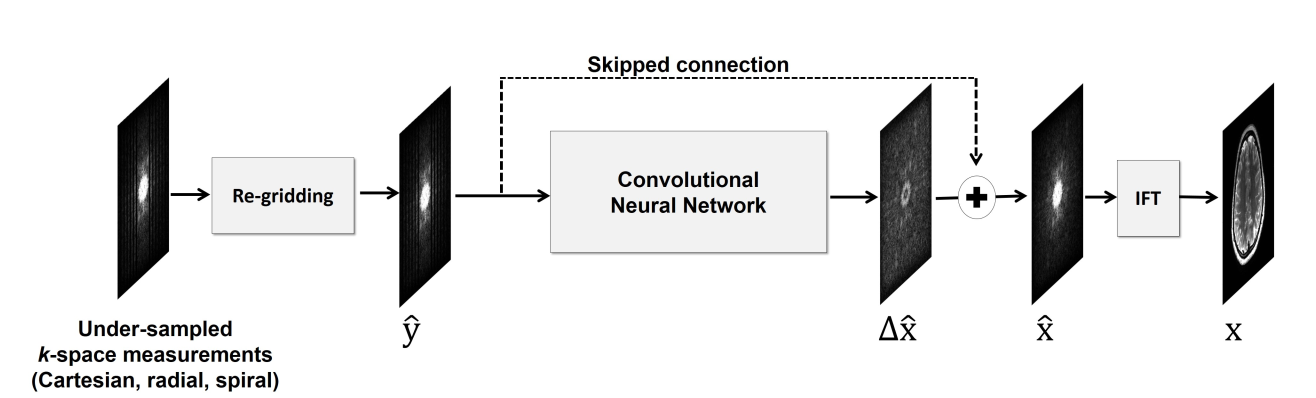
\includegraphics[width=0.7\linewidth]{chapters/chapter-3/figs/kspace2020-Architecture-a}
		\label{subfig:kspace2020-architecture-a}
	}
	\subfigure[]{
		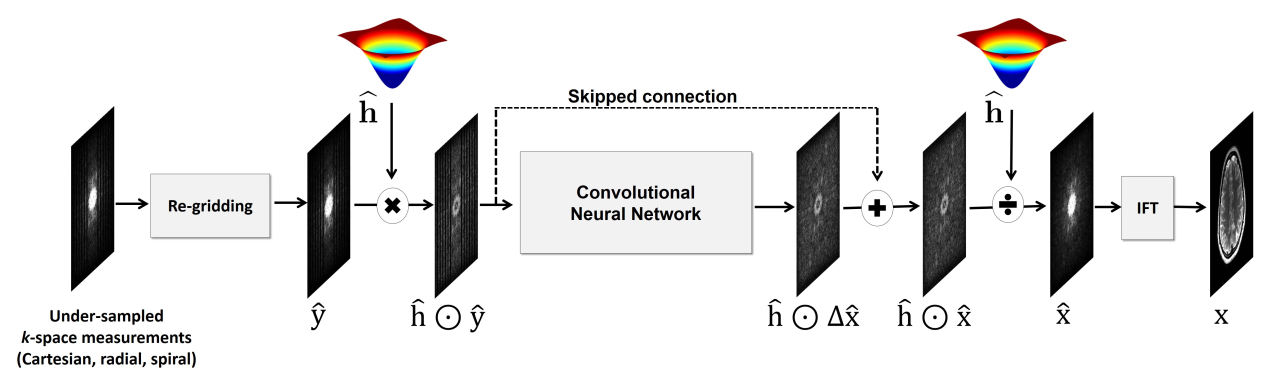
\includegraphics[width=0.7\linewidth]{chapters/chapter-3/figs/kspace2020-Architecture-b}
		\label{subfig:kspace2020-architecture-b}
	}
	\label{fig:kspace2020-architectures}
\end{figure}

توجه داریم که در ساختار های \ref{fig:kspace2020-architectures}
از اسکیپ کاننکشن 
\LTRfootnote{Skip-Connection}
استفاده کرده است. این اسکیپ کانکشن کمک به ایجاد یک ساختار \lr{Residual} و تولید ساختار های اسپارس تر در ورودی شبکه یادگیری عمیق است. بنابراین به اسپارسیتی ورودی آن افزوده میشود.

برای ساختار اتوانکودر نیز از ساختار معروف \lr{UNET} استفاده شده است که تصویر 
\ref{fig:unet}
این ساختار متقارن و داری اسکیپ کانکشن های خود را نشان میدهد که بعنوان اتوانکودر بسیار کاربرد دارد.



\begin{figure}
	\centering
	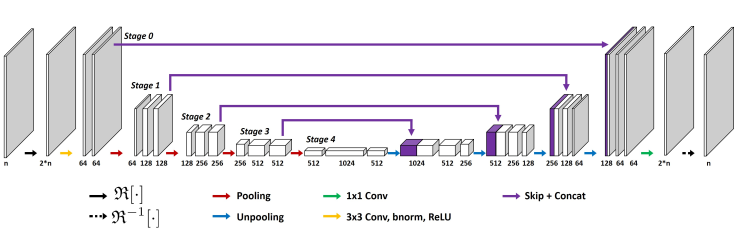
\includegraphics[width=0.9\linewidth]{chapters/chapter-3/figs/unet}
	\caption{}
	\label{fig:unet}
\end{figure}









